\section{USART Unit}

The \gls{USART} unit provides access to one of the microcontroller's \gls{USART} peripherals. See \cref{sec:theory_usart} for more information about the interface.

Most \gls{USART} parameters available in the hardware peripheral's configuration registers can be adjusted to match the application's needs. The peripheral is capable of driving RS-485 transceivers, using the \gls{DE} output for switching between reception and transmission.

The unit implements asynchronous reception and transmission with \gls{DMA} and a circular buffer (\cref{fig:uart_rx_dma}). Received data is sent to the host in asynchronous events when a half of the buffer is filled, or after a fixed timeout from the last received byte. The write access is, likewise, implemented using a \gls{DMA} buffer.

\begin{figure}[h]
	\centering
	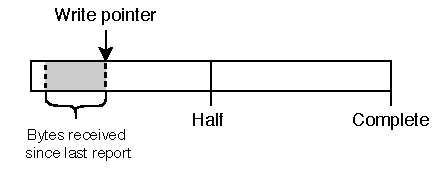
\includegraphics[scale=1]{img/uart-dma.pdf}
	\caption{\label{fig:uart_rx_dma}Principle of DMA-based UART reception. Interrupt is generated in the half and at the end of the buffer, at which point the write pointer wraps back to the beginning.}
\end{figure}

\subsection{USART Configuration}

\begin{inicode}
[USART:ser@6]
# Peripheral number (UARTx 1-4)
device=1
# Pin mappings (TX,RX,CK,CTS,RTS/DE)
#  USART1: (0) A9,A10,A8,A11,A12   (1) B6,B7,A8,A11,A12
#  USART2: (0) A2,A3,A4,A0,A1      (1) A14,A15,A4,A0,A1
#  USART3: (0) B10,B11,B12,B13,B14
#  USART4: (0) A0,A1,C12,B7,A15    (1) C10,C11,C12,B7,A15
remap=0

# Baud rate in bps (eg. 9600)
baud-rate=115200
# Parity type (NONE, ODD, EVEN)
parity=NONE
# Number of stop bits (0.5, 1, 1.5, 2)
stop-bits=1
# Bit order (LSB or MSB first)
first-bit=LSB
# Word width (7,8,9) - including parity bit if used
word-width=8
# Enabled lines (RX,TX,RXTX)
direction=RXTX
# Hardware flow control (NONE, RTS, CTS, FULL)
hw-flow-control=NONE

# Generate serial clock (Y,N)
clock-output=N
# Clock polarity: 0,1
cpol=0
# Clock phase: 0,1
cpha=0

# Generate RS485 Driver Enable signal (Y,N) - uses RTS pin
de-output=N
# DE active level: 0,1
de-polarity=1
# DE assert time (0-31)
de-assert-time=8
# DE clear time (0-31)
de-clear-time=8
\end{inicode}


\subsection{USART Events}

\begin{cmdlist}

	0 & \cname{DATA\_RECEIVED}
	Data was received on the serial port.
	&
    \begin{cmdpld}
		\cfield{u8[]} received bytes
    \end{cmdpld} \\

\end{cmdlist}


\subsection{USART Commands}

\begin{cmdlist}

	0 & \cname{WRITE}
	Add data to the transmit buffer. Sending is asynchronous, but the command may wait for free space in the \gls{DMA} buffer.
	& \begin{cmdreq}
		\cfield{u8[]} bytes to write
    \end{cmdreq} \\

	1 & \cname{WRITE\_SYNC}
	Add data to the transmit buffer and wait for the transmission to complete.
	& \begin{cmdreq}
		\cfield{u8[]} bytes to write
    \end{cmdreq} \\

\end{cmdlist}










